
\section{Monitoring of the Front End Electronics}

\gls{FEE} monitoring plays a crucial role in the detector operation, but also during the testing phase. Internal parameters of the \glspl{ASIC} in the \gls{ROB} or \gls{FEB} deliver information about the stability and onset of failure.


The first application of the introduced control framework was to read out several parameters from different readout chains (see section \ref{readout} for a detailed explanation of different readout chains). The \gls{ROB} and \gls{DPB} based readout chain were used to evaluate the possibility of interfacing the values from the \gls{DAQ} chain to the slow control and \gls{EPICS} based system.

The purpose was to monitor the stability of the readouts throughout different tests, e.g. during the thermal cycling of \gls{FEE}. A similar interface was also developed for the GBTemu readout chain. 

Two \glspl{FEB} - 16 STS-XYTERs were used to evaluate the performance of the intarface and the ASICs. It constitutes to in total 112 process variables, which makes it a relatively small setup. Those values were then stored in a database and are available from Phoebus for further analysis and visualization.

To get the values from the \glspl{ASIC} a soft \gls{IOC} with a pyEPICS~\cite{pyEPICS} interface was used. The monitoring studies included the registers and corresponding values available from \gls{GBT} \gls{SCA2} \gls{ASIC} \cite{GBT_SCA_ASIC} and three GBTX chips: 
\begin{itemize}
    \item GBT SCA - RSSI (Received Single Strength Indicator), input voltage $V_{in}$, 1.5~V DC/DC converter output voltage $V_{out}$, 2.5~V DC/DC converter output voltage $V_{out}$ (see figure~\ref{fig:ROB}), two temperature sensors,
    \item GBTX \gls{ASIC} - FEC (Forward Error Correction) counts.
\end{itemize}
%\newpage

\begin{figure}[!h]
    \centering
    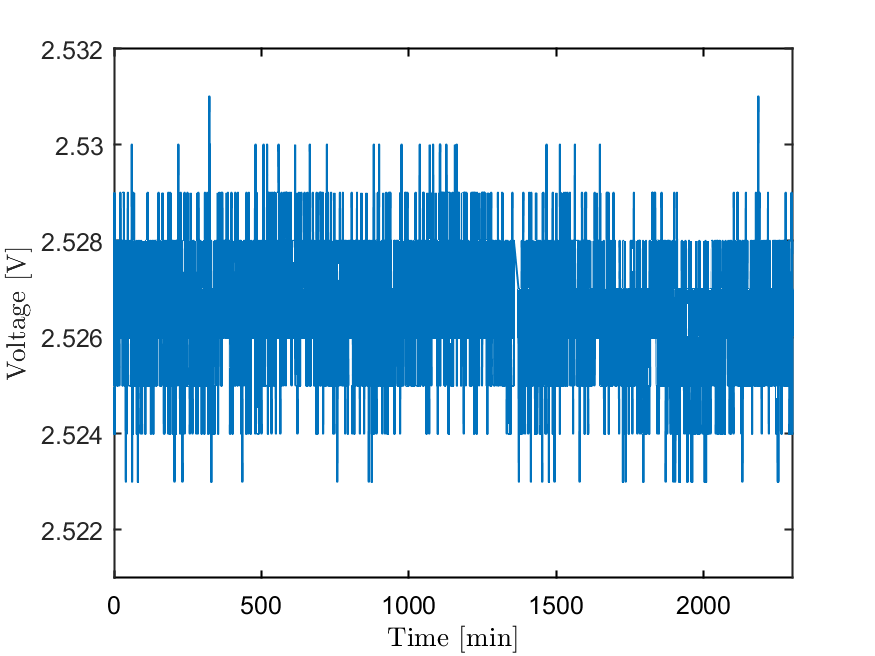
\includegraphics[width=0.65\columnwidth]{Chapter4/images/ROB.png}
    \caption{$V_{out}$ output voltage from one of the DC/DC converters in the \gls{ROB}}
    \label{fig:ROB}
\end{figure}

The STS-XYTER provides the following values - almost full counter, event missed counter, single event upset counter, the status register, and \gls{DAC} values: $V_{ddm}$, \gls{CSA} bias, temperature. 

\begin{figure}[!h]
    \centering
    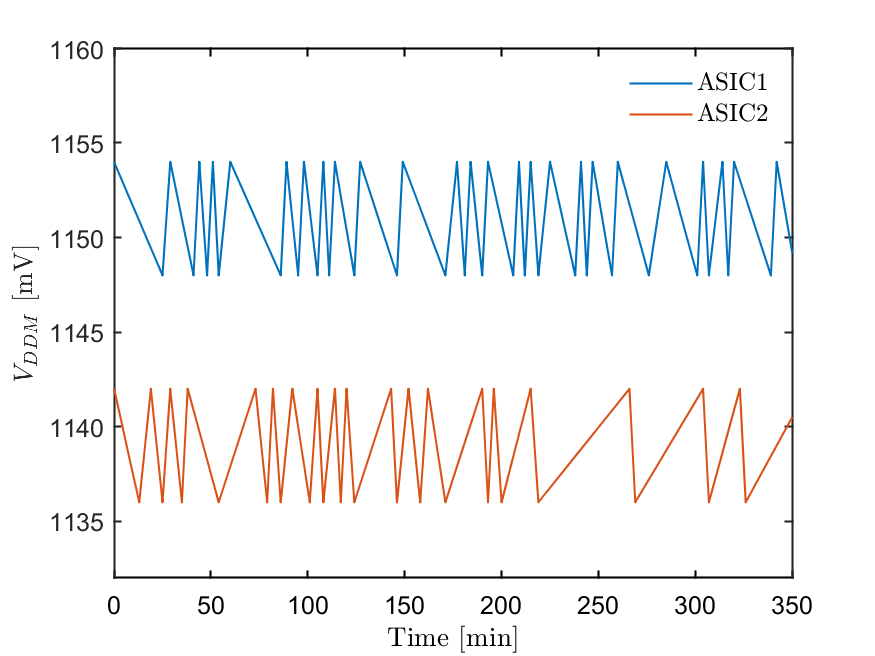
\includegraphics[width=0.65\columnwidth]{Chapter4/images/FEB.png}
    \caption{$V_{ddm}$ readouts from the diagnostic circuits of two ASICs}
    \label{fig:vddm_first}
\end{figure}

%\subsection{Parameters of the STS-XYTERv2 ASIC}
%\subsection{GBTX and GBT ASIC monitoring}